\documentclass{article}\usepackage[]{graphicx}\usepackage[]{xcolor}
% maxwidth is the original width if it is less than linewidth
% otherwise use linewidth (to make sure the graphics do not exceed the margin)
\makeatletter
\def\maxwidth{ %
  \ifdim\Gin@nat@width>\linewidth
    \linewidth
  \else
    \Gin@nat@width
  \fi
}
\makeatother

\definecolor{fgcolor}{rgb}{0.345, 0.345, 0.345}
\newcommand{\hlnum}[1]{\textcolor[rgb]{0.686,0.059,0.569}{#1}}%
\newcommand{\hlsng}[1]{\textcolor[rgb]{0.192,0.494,0.8}{#1}}%
\newcommand{\hlcom}[1]{\textcolor[rgb]{0.678,0.584,0.686}{\textit{#1}}}%
\newcommand{\hlopt}[1]{\textcolor[rgb]{0,0,0}{#1}}%
\newcommand{\hldef}[1]{\textcolor[rgb]{0.345,0.345,0.345}{#1}}%
\newcommand{\hlkwa}[1]{\textcolor[rgb]{0.161,0.373,0.58}{\textbf{#1}}}%
\newcommand{\hlkwb}[1]{\textcolor[rgb]{0.69,0.353,0.396}{#1}}%
\newcommand{\hlkwc}[1]{\textcolor[rgb]{0.333,0.667,0.333}{#1}}%
\newcommand{\hlkwd}[1]{\textcolor[rgb]{0.737,0.353,0.396}{\textbf{#1}}}%
\let\hlipl\hlkwb

\usepackage{framed}
\makeatletter
\newenvironment{kframe}{%
 \def\at@end@of@kframe{}%
 \ifinner\ifhmode%
  \def\at@end@of@kframe{\end{minipage}}%
  \begin{minipage}{\columnwidth}%
 \fi\fi%
 \def\FrameCommand##1{\hskip\@totalleftmargin \hskip-\fboxsep
 \colorbox{shadecolor}{##1}\hskip-\fboxsep
     % There is no \\@totalrightmargin, so:
     \hskip-\linewidth \hskip-\@totalleftmargin \hskip\columnwidth}%
 \MakeFramed {\advance\hsize-\width
   \@totalleftmargin\z@ \linewidth\hsize
   \@setminipage}}%
 {\par\unskip\endMakeFramed%
 \at@end@of@kframe}
\makeatother

\definecolor{shadecolor}{rgb}{.97, .97, .97}
\definecolor{messagecolor}{rgb}{0, 0, 0}
\definecolor{warningcolor}{rgb}{1, 0, 1}
\definecolor{errorcolor}{rgb}{1, 0, 0}
\newenvironment{knitrout}{}{} % an empty environment to be redefined in TeX

\usepackage{alltt}
\usepackage[margin=1.0in]{geometry} % To set margins
\usepackage{amsmath}  % This allows me to use the align functionality.
                      % If you find yourself trying to replicate
                      % something you found online, ensure you're
                      % loading the necessary packages!
\usepackage{amsfonts} % Math font
\usepackage{fancyvrb}
\usepackage{hyperref} % For including hyperlinks
\usepackage[shortlabels]{enumitem}% For enumerated lists with labels specified
                                  % We had to run tlmgr_install("enumitem") in R
\usepackage{float}    % For telling R where to put a table/figure
\usepackage{natbib}        %For the bibliography
\bibliographystyle{apalike}%For the bibliography
\IfFileExists{upquote.sty}{\usepackage{upquote}}{}
\begin{document}


\cite{Kasdin25} show that dopamine in the brains of young zebra finches acts as 
a learning signal, increasing when they sing closer to their adult song and 
decreasing when they sing further away, effectively guiding their vocal 
development through trial-and-error. This suggests that complex natural 
behaviors, like learning to sing, are shaped by dopamine-driven reinforcement 
learning, similar to how artificial intelligence learns. You can find the 
paper at this link:
\href{https://www.nature.com/articles/s41586-025-08729-1}{{https://www.nature.com/articles/s41586-025-08729-1}.}.

Note they measure dopamine using fibre photometry, changes in the fluorescence
indicate dopamine changes in realtime. Their specific measurement considers 
changes in flourescence in 100-ms windows between 200 and 300 ms from the start 
of singing, averaged across development.

\begin{enumerate}
%%%%%%%%%%%%%%%%%%%%%%%%%%%%%%%%%%%%%%%%%%%%%%%%%%%%%%%%%%%%%%%%%
% CONDUCT A POWER ANALYSIS
%%%%%%%%%%%%%%%%%%%%%%%%%%%%%%%%%%%%%%%%%%%%%%%%%%%%%%%%%%%%%%%%%

\item Using the \texttt{pwr} package for \texttt{R} \citep{pwr},
conduct a power analysis. How many observations would the researchers 
need to detect a moderate-to-large effect ($d=0.65$) when using 
$\alpha=0.05$ and default power (0.80) for a two-sided one sample 
$t$ test. - \textbf{The researchers would need approximately 21 observations in order to detect a moderate-to-large effect while using the parameters listed above.}

\begin{knitrout}\scriptsize
\definecolor{shadecolor}{rgb}{0.969, 0.969, 0.969}\color{fgcolor}\begin{kframe}
\begin{alltt}
\hlkwd{library}\hldef{(pwr)}
\end{alltt}


{\ttfamily\noindent\color{warningcolor}{\#\# Warning: package 'pwr' was built under R version 4.4.3}}\begin{alltt}
\hlkwd{library}\hldef{(effectsize)}
\end{alltt}


{\ttfamily\noindent\color{warningcolor}{\#\# Warning: package 'effectsize' was built under R version 4.4.3}}\begin{alltt}
\hlkwd{suppressPackageStartupMessages}\hldef{(}\hlkwd{library}\hldef{(tidyverse))}
\hlkwd{library}\hldef{(patchwork)}
\hlcom{###Question 1: Use pwr to find # of obs needed to detect mod to lrg effect}
\hldef{num.obs} \hlkwb{<-} \hlkwd{pwr.t.test}\hldef{(}\hlkwc{n}\hldef{=}\hlkwa{NULL}\hldef{,} \hlkwc{d} \hldef{=} \hlnum{0.65}\hldef{,} \hlkwc{sig.level} \hldef{=} \hlnum{0.05}\hldef{,} \hlkwc{power} \hldef{=} \hlnum{0.80}\hldef{,} \hlkwc{type}\hldef{=}\hlsng{"one.sample"}\hldef{)}
\end{alltt}
\end{kframe}
\end{knitrout}
%%%%%%%%%%%%%%%%%%%%%%%%%%%%%%%%%%%%%%%%%%%%%%%%%%%%%%%%%%%%%%%%%
% COLLECT DATA
%%%%%%%%%%%%%%%%%%%%%%%%%%%%%%%%%%%%%%%%%%%%%%%%%%%%%%%%%%%%%%%%%
\item Click the link to go to the paper. Find the source data for 
Figure 2. Download the Excel file. Describe what you needed to
do to collect the data for Figure 2(g). Note that you only need the 
\texttt{closer\_vals} and \texttt{further\_vals}. Ensure to 
\texttt{mutate()} the data to get a difference 
(e.g., \texttt{closer\_vals - further\_vals}). - \textbf{In order to collect the data from the paper, I first had to download the xlsx file from the source data provided within the paper, and then copy it into a blank csv file so that it could be read by R.}
%%%%%%%%%%%%%%%%%%%%%%%%%%%%%%%%%%%%%%%%%%%%%%%%%%%%%%%%%%%%%%%%%
% SUMMARIZE DATA
%%%%%%%%%%%%%%%%%%%%%%%%%%%%%%%%%%%%%%%%%%%%%%%%%%%%%%%%%%%%%%%%%
\item Summarize the data.
\begin{enumerate}
  \item Summarize the further data. Do the data suggest that
   dopamine in the brains of young zebra finches decreases when
   they sing further away? - \textbf{The data suggests that the dopamine in the brains of young zebra finches does decrease when the song they sing is further from their addult song as all of the observations display a negative change in flourescence for birds who were further from their adult songs.}
\begin{knitrout}\scriptsize
\definecolor{shadecolor}{rgb}{0.969, 0.969, 0.969}\color{fgcolor}\begin{kframe}
\begin{alltt}
\hldef{fig2data} \hlkwb{<-} \hlkwd{read.csv}\hldef{(}\hlsng{"cleandata.csv"}\hldef{)}
\hldef{further.sum} \hlkwb{<-} \hldef{fig2data |>}
\hlkwd{summarize}\hldef{(}
  \hlkwc{mean} \hldef{=} \hlkwd{mean}\hldef{(further.vals,} \hlkwc{na.rm} \hldef{=} \hlnum{TRUE}\hldef{),}
  \hlkwc{sd} \hldef{=} \hlkwd{sd}\hldef{(further.vals,} \hlkwc{na.rm} \hldef{=} \hlnum{TRUE}\hldef{)}
\hldef{)}
\hldef{further.sum}
\end{alltt}
\begin{verbatim}
##         mean        sd
## 1 -0.2031844 0.1331014
\end{verbatim}
\end{kframe}
\end{knitrout}
   \item Summarize the closer data. Do the data suggest that
   dopamine in the brains of young zebra finches increases when
   they sing closer to their adult song? - \textbf{The data suggests that the dopamine in the brains of young zebra finches does increase when the song they sing is closer to their addult song as most of the observations display a positive change in flourescence for birds who were closer to their adult songs.}
\begin{knitrout}\scriptsize
\definecolor{shadecolor}{rgb}{0.969, 0.969, 0.969}\color{fgcolor}\begin{kframe}
\begin{alltt}
\hldef{closer.sum} \hlkwb{<-} \hldef{fig2data |>}
  \hlkwd{summarize}\hldef{(}
 \hlkwc{mean} \hldef{=} \hlkwd{mean}\hldef{(further.vals,} \hlkwc{na.rm} \hldef{=} \hlnum{TRUE}\hldef{),}
 \hlkwc{sd} \hldef{=} \hlkwd{sd}\hldef{(further.vals,} \hlkwc{na.rm} \hldef{=} \hlnum{TRUE}\hldef{)}
  \hldef{)}
\hldef{closer.sum}
\end{alltt}
\begin{verbatim}
##         mean        sd
## 1 -0.2031844 0.1331014
\end{verbatim}
\end{kframe}
\end{knitrout}
  \item Summarize the paired differences. Do the data suggest
  that there is a difference between dopamine in the brains of
  young zebra finches when they sing further away compared to 
  closer to their adult song? - \textbf{The data does suggest that there is a difference in finches who sing further away from their adult song than ones who sing closer to it as the difference between the two values remains positive for all observations.}
\begin{knitrout}\scriptsize
\definecolor{shadecolor}{rgb}{0.969, 0.969, 0.969}\color{fgcolor}\begin{kframe}
\begin{alltt}
\hldef{diff.sum} \hlkwb{<-} \hldef{fig2data |>}
\hlkwd{summarize}\hldef{(}
  \hlkwc{mean} \hldef{=} \hlkwd{mean}\hldef{(difference,} \hlkwc{na.rm} \hldef{=} \hlnum{TRUE}\hldef{),}
  \hlkwc{sd} \hldef{=} \hlkwd{sd}\hldef{(difference,} \hlkwc{na.rm} \hldef{=} \hlnum{TRUE}\hldef{)}
\hldef{)}
\hldef{diff.sum}
\end{alltt}
\begin{verbatim}
##        mean        sd
## 1 0.3544287 0.2141698
\end{verbatim}
\end{kframe}
\end{knitrout}
\begin{figure}[H]
\begin{center}
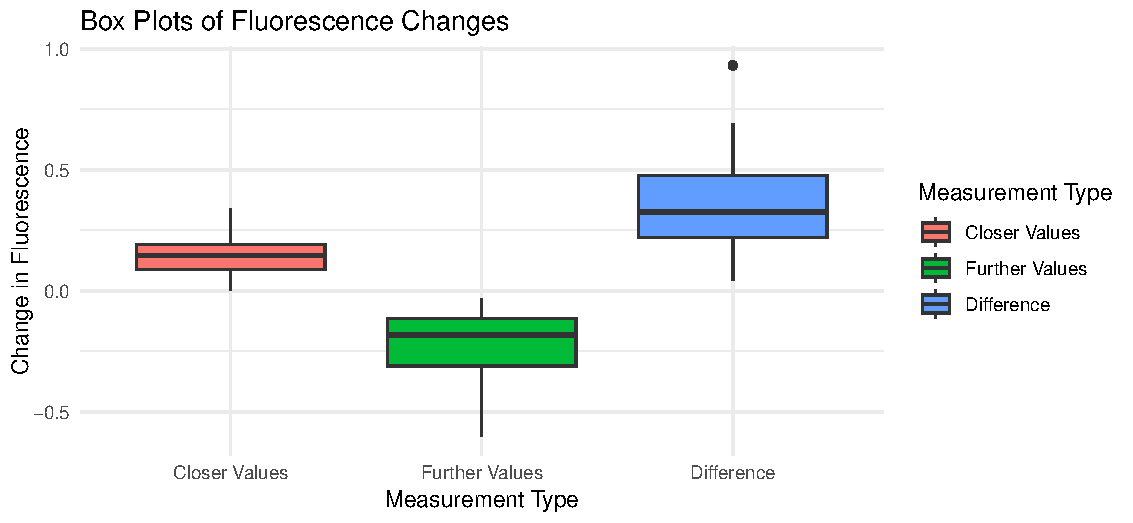
\includegraphics[scale=0.5]{graphicalsummaries.pdf}
\label{plot1}
\end{center}
\end{figure}
  \item \textbf{Optional Challenge:} Can you reproduce Figure 2(g)?
  Note that the you can use \texttt{geom\_errorbar()} to plot
  the range created by adding the mean $\pm$ one standard deviation.
\end{enumerate}
%%%%%%%%%%%%%%%%%%%%%%%%%%%%%%%%%%%%%%%%%%%%%%%%%%%%%%%%%%%%%%%%%
% CONDUCT THE TESTS
%%%%%%%%%%%%%%%%%%%%%%%%%%%%%%%%%%%%%%%%%%%%%%%%%%%%%%%%%%%%%%%%%
\item Conduct the inferences they do in the paper. Make sure to report the results
a little more comprehensively -- that is your parenthetical should look something
like: ($t=23.99$, $p<0.0001$; $g=1.34$; 95\% CI: 4.43, 4.60).\\
\textbf{Note:} Your numbers may vary slightly as they performed some unclear
correction of their $p$-values. I'm waiting to hear back from them via email!
\begin{enumerate}
  \item ``The close responses differed significantly from 0 ($p=1.63 \times 10^{-8}$).'' - The close finch responses differed significantly from 0 and suggest a large effect size ($t=7.9945$, $p=4.34 \times  10^{-8}$; $g=1.34$; 95\% CI: 0.97, 2.17)
\begin{knitrout}\scriptsize
\definecolor{shadecolor}{rgb}{0.969, 0.969, 0.969}\color{fgcolor}\begin{kframe}
\begin{alltt}
\hldef{mu0} \hlkwb{=} \hlnum{0}
\hldef{x} \hlkwb{<-} \hldef{fig2data}\hlopt{$}\hldef{closer.vals}
\hldef{y} \hlkwb{<-} \hldef{fig2data}\hlopt{$}\hldef{further.vals}
\hldef{z} \hlkwb{<-} \hldef{fig2data}\hlopt{$}\hldef{difference}
\hldef{(xbar} \hlkwb{<-} \hlkwd{mean}\hldef{(x))}
\end{alltt}
\begin{verbatim}
## [1] 0.1512443
\end{verbatim}
\begin{alltt}
\hldef{(s} \hlkwb{<-} \hlkwd{sd}\hldef{(x))}
\end{alltt}
\begin{verbatim}
## [1] 0.09268119
\end{verbatim}
\begin{alltt}
\hldef{(n} \hlkwb{<-} \hlkwd{length}\hldef{(x))}
\end{alltt}
\begin{verbatim}
## [1] 24
\end{verbatim}
\begin{alltt}
\hlkwd{any}\hldef{(}\hlkwd{is.na}\hldef{(x))}
\end{alltt}
\begin{verbatim}
## [1] FALSE
\end{verbatim}
\begin{alltt}
\hldef{x.hedges} \hlkwb{<-} \hlkwd{hedges_g}\hldef{(}\hlkwc{x} \hldef{= x,} \hlkwc{mu} \hldef{= mu0,} \hlkwc{alternative} \hldef{=} \hlsng{"two.sided"}\hldef{)}
\hlkwd{interpret_hedges_g}\hldef{(}\hlnum{1.34}\hldef{)}
\end{alltt}
\begin{verbatim}
## [1] "large"
## (Rules: cohen1988)
\end{verbatim}
\begin{alltt}
\hldef{close.t.stat} \hlkwb{<-} \hlkwd{t.test}\hldef{(}\hlkwc{x}\hldef{=x,} \hlkwc{mu} \hldef{= mu0,} \hlkwc{alternative} \hldef{=} \hlsng{"two.sided"}\hldef{)}
\hldef{x.hedges}
\end{alltt}
\begin{verbatim}
## Hedges' g |       95% CI
## ------------------------
## 1.58      | [0.97, 2.17]
\end{verbatim}
\begin{alltt}
\hldef{close.t.stat}
\end{alltt}
\begin{verbatim}
## 
## 	One Sample t-test
## 
## data:  x
## t = 7.9945, df = 23, p-value = 4.34e-08
## alternative hypothesis: true mean is not equal to 0
## 95 percent confidence interval:
##  0.1121084 0.1903801
## sample estimates:
## mean of x 
## 0.1512443
\end{verbatim}
\end{kframe}
\end{knitrout}
  \item ``The far responses differed significantly from 0 ($p=5.17 \times 10^{-8}$).''  - The further finch responses differed significantly from 0 and suggest a large effect size ($t=-7.4785$, $p=1.34 \times  10^{-7}$; $g=-1.48$; 95\% CI: -2.04, -0.89)
\begin{knitrout}\scriptsize
\definecolor{shadecolor}{rgb}{0.969, 0.969, 0.969}\color{fgcolor}\begin{kframe}
\begin{alltt}
\hldef{y.hedges} \hlkwb{<-} \hlkwd{hedges_g}\hldef{(}\hlkwc{x} \hldef{= y,} \hlkwc{mu} \hldef{= mu0,} \hlkwc{alternative} \hldef{=} \hlsng{"two.sided"}\hldef{)}
\hlkwd{interpret_hedges_g}\hldef{(}\hlopt{-}\hlnum{1.48}\hldef{)}
\end{alltt}
\begin{verbatim}
## [1] "large"
## (Rules: cohen1988)
\end{verbatim}
\begin{alltt}
\hldef{far.t.stat} \hlkwb{<-} \hlkwd{t.test}\hldef{(}\hlkwc{x}\hldef{=y,} \hlkwc{mu} \hldef{= mu0,} \hlkwc{alternative} \hldef{=} \hlsng{"two.sided"}\hldef{)}
\hldef{y.hedges}
\end{alltt}
\begin{verbatim}
## Hedges' g |         95% CI
## --------------------------
## -1.48     | [-2.04, -0.89]
\end{verbatim}
\begin{alltt}
\hldef{far.t.stat}
\end{alltt}
\begin{verbatim}
## 
## 	One Sample t-test
## 
## data:  y
## t = -7.4785, df = 23, p-value = 1.337e-07
## alternative hypothesis: true mean is not equal to 0
## 95 percent confidence interval:
##  -0.2593882 -0.1469806
## sample estimates:
##  mean of x 
## -0.2031844
\end{verbatim}
\end{kframe}
\end{knitrout}
  \item ``The difference between populations was significant ($p=1.04 \times10^{-8}$).'' - The difference between closer and further finch responses differed significantly from one another and suggest a large effect size ($t=8.1073$, $p=3.41 \times  10^{-8}$; $g=1.6$; 95\% CI: 0.99, 2.19).
\begin{knitrout}\scriptsize
\definecolor{shadecolor}{rgb}{0.969, 0.969, 0.969}\color{fgcolor}\begin{kframe}
\begin{alltt}
\hldef{z.hedges} \hlkwb{<-} \hlkwd{hedges_g}\hldef{(}\hlkwc{x} \hldef{= z,} \hlkwc{mu} \hldef{= mu0,} \hlkwc{alternative} \hldef{=} \hlsng{"two.sided"}\hldef{)}
\hlkwd{interpret_hedges_g}\hldef{(}\hlnum{1.60}\hldef{)}
\end{alltt}
\begin{verbatim}
## [1] "large"
## (Rules: cohen1988)
\end{verbatim}
\begin{alltt}
\hldef{diff.t.stat} \hlkwb{<-} \hlkwd{t.test}\hldef{(}\hlkwc{x}\hldef{=z,} \hlkwc{mu} \hldef{= mu0,} \hlkwc{alternative} \hldef{=} \hlsng{"two.sided"}\hldef{)}
\hldef{z.hedges}
\end{alltt}
\begin{verbatim}
## Hedges' g |       95% CI
## ------------------------
## 1.60      | [0.99, 2.19]
\end{verbatim}
\begin{alltt}
\hldef{diff.t.stat}
\end{alltt}
\begin{verbatim}
## 
## 	One Sample t-test
## 
## data:  z
## t = 8.1073, df = 23, p-value = 3.41e-08
## alternative hypothesis: true mean is not equal to 0
## 95 percent confidence interval:
##  0.2639927 0.4448646
## sample estimates:
## mean of x 
## 0.3544287
\end{verbatim}
\end{kframe}
\end{knitrout}
\end{enumerate}
%%%%%%%%%%%%%%%%%%%%%%%%%%%%%%%%%%%%%%%%%%%%%%%%%%%%%%%%%%%%%%%%%
% CONDUCT THE TESTS
%%%%%%%%%%%%%%%%%%%%%%%%%%%%%%%%%%%%%%%%%%%%%%%%%%%%%%%%%%%%%%%%%
\item Reverse engineer the hypothesis test plot from Lecture 20 to create accurate
hypothesis testing plots for each part of the previous question.
\begin{enumerate}
  \item Question 4, part(a).
  \item Question 4, part(b).
  \item Question 4, part(c).
  \begin{figure}[H]
\begin{center}
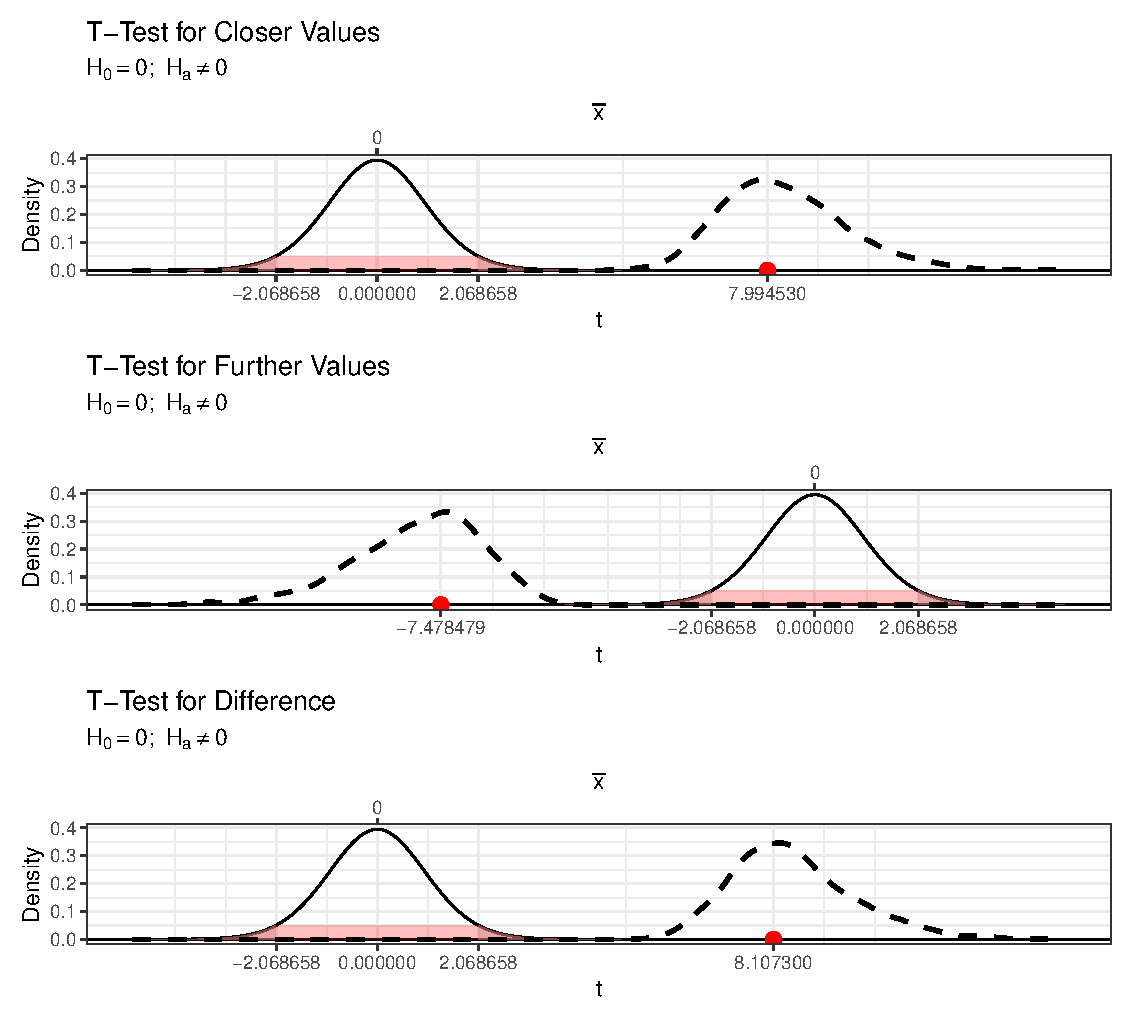
\includegraphics[scale=0.5]{Rplot.pdf}
\label{plot2}
\end{center}
\end{figure}
\end{enumerate}
\end{enumerate}


\bibliography{bibliography}
\end{document}
